\section{UPPAAL}
\begin{frame}[shrink=5]{UPPAAL}
    \begin{center}
        \scalebox{0.9}{
    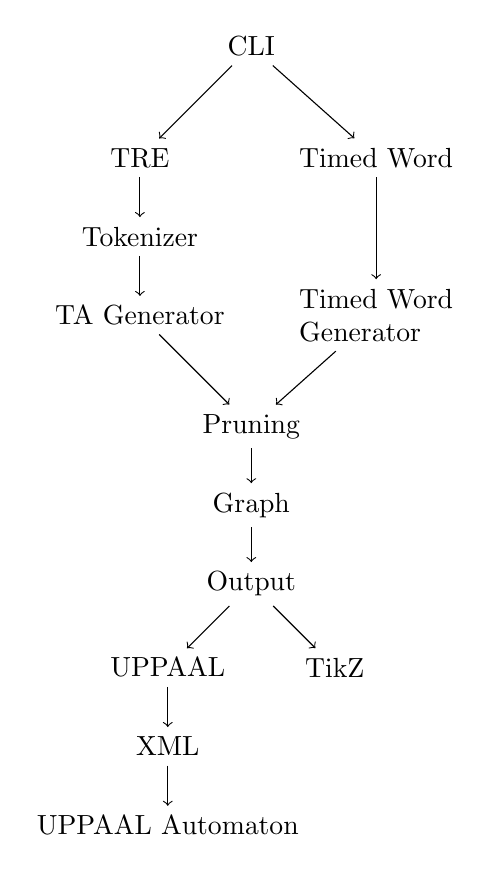
\begin{tikzpicture}[node distance = 1cm, auto]\label{fig:TREATdiagram}
        \node (CLI) {CLI};
        
        \node (TRE) [node distance = 2cm, below left of = CLI] {TRE};
        \node (TimedWord) [node distance = 3cm, right of = TRE] {Timed Word};
        \node (Tokenizer) [below of = TRE] {Tokenizer};
        \node (TAGenerator) [below of = Tokenizer] {TA Generator};
        \node (Pruning) [node distance = 2cm, below right of = TAGenerator] {Pruning};
        \node (Graph) [below of = Pruning] {Graph};
        \node (Output) [below of = Graph] {Output};
        \node (UPPAAL) [node distance = 1.5cm, below left of = Output] {UPPAAL};
        \node (XML) [below of = UPPAAL] {XML};
        \node (UPPAALAutomaton) [below of = XML] {UPPAAL Automaton};
        \node (TikZ) [node distance = 1.5cm, below right of = Output] {TikZ};
        \node (TimedWordGenerator) [node distance = 3cm, right of = TAGenerator,  align=left] {Timed Word\\Generator};
    
        \draw[->] (CLI) -- (TRE);
        \draw[->] (TRE) -- (Tokenizer);
        \draw[->] (Tokenizer) -- (TAGenerator);
        \draw[->] (TAGenerator) -- (Pruning);
        \draw[->] (Pruning) -- (Graph);
        \draw[->] (Graph) -- (Output);
        \draw[->] (Output) -- (UPPAAL);
        \draw[->] (UPPAAL) -- (XML);
        \draw[->] (XML) -- (UPPAALAutomaton);
        \draw[->] (Output) -- (TikZ);
        \draw[->] (CLI) -- (TimedWord);
        \draw[->] (TimedWord) -- (TimedWordGenerator);
        \draw[->] (TimedWordGenerator) -- (Pruning);
    \end{tikzpicture}
}

    \end{center}
\end{frame}
\begin{frame}{UPPAAL}
    \begin{columns}
        \begin{column}{0.4\textwidth}
            \begin{itemize}
                \item UML
                \item Structured using UPPAAL .dtd
            \end{itemize}
        \end{column}
        \begin{column}{0.6\textwidth}
            \scalebox{0.8}{
                \scalebox{0.8}{
\begin{tikzpicture}
        \umlclass[anchor=north,width=31ex,x=0,y=0]{nta}{declaration : string\\system : string}{}

        %classes
        \umlclass[anchor=north,width=31ex,x=0,y=-4.3]{template}{declaration : string\\name : string\\ init : string}{}
        %relations
        \umlcompo[attr1=1|,attr2=0..*|,pos2=0.87]{nta}{template}

        %classes
        %\umlclass[x=-6,y=-6]{parameter}{}{}
        %\umlclass[x=-3,y=-6]{branchpoint}{}{}
        \umlclass[anchor=north,width=31ex,x=0,y=-9]{location}{id : string\\name : string\\label : List$<$(string, string)$>$}{}
        \umlclass[anchor=north,width=31ex,x=6,y=-9]{transition}{id : string\\source : string\\target : string\\label : List$<$(string, string)$>$}{}
        %\umlclass[x=15,y=-6]{parameter}{}{}
        %relations
        \umlcompo[attr1=1|,attr2=0..*|,pos1=0.15,pos2=0.9]{template}{location}
        \umlHVcompo[attr1=1|,attr2=0..*|,pos1=0.1,pos2=1.95]{template}{transition}
        %\umlVHVcompo[attr2=0..1|,pos2=2.75]{template}{parameter}

        %classes
        %\umlclass[x=-6,y=-9]{committed}{}{}
        %\umlclass[x=-9,y=-9]{urgent}{}{}
        %relations
        %\umlVHVcompo[attr2=0..1|,pos2=2.75]{location}{committed}
        %\umlVHVcompo[attr2=0..1|,pos2=2.75]{location}{urgent}
    \end{tikzpicture}}


            }
        \end{column}
    \end{columns}
    % \hspace{10em}

\end{frame}
\begin{frame}[fragile]{UPPAAL}

    \begin{lstlisting}[style=csharp]
internal Nta()
{
    _templates = new List<Template>();
    Declaration = new Declaration(new List<string>(), new List<string>());
}    
    \end{lstlisting}
    \vspace{1em}
    \begin{lstlisting}[style=csharp]
internal Template(...)
{
    Declaration = declaration;
    Declaration.AddClocks(clocks);
    Name = name;
    Init = init;
    _locations = locations.ToArray();
    _transitions = transitions.ToArray();
}  
    \end{lstlisting}
\end{frame}

\begin{frame}{Demonstration}
    \begin{columns}
        \begin{column}{0.4\textwidth}
            \begin{itemize}
                \item UPPAAL
                \item TikZ
                \item Queries
            \end{itemize}
        \end{column}
        \begin{column}{0.6\textwidth}
            \visible<2>{
                
\includegraphics[width=\columnwidth, keepaspectratio]{Documents/thumb.png}
            }

        \end{column}
    \end{columns}
\end{frame}

\section{Discussion}
\begin{frame}{Future works}
    \begin{columns}
        \begin{column}{0.4\textwidth}
            \begin{itemize}
                \item Pruning
                \item <4>TA $\rightarrow$ TRE
            \end{itemize}
        \end{column}
        \begin{column}{0.6\textwidth}
            \visible<2-3> {
                \scalebox{0.8}{
                    \begin{tikzpicture}[auto]
                        \node[state, accepting] at (2, 0)(q0){$q0$};
                        \node[state] at (2, 2)(q1){$q1$};
                        \node[state, accepting] at (5, 0)(q2){$q2$};
                        \node[state, initial] at (0, 0)(q3){$q3$};

                        \path[->]
                        (q1)edge node{$A$}(q2)
                        (q3)edge node{$A$}(q0)
                        (q3)edge node{$B$}(q1)
                        ;
                    \end{tikzpicture}
                }
            }

            \vspace{2em}
            \visible<3> {
                \scalebox{0.8}{
                    \begin{tikzpicture}[auto]
                        \node[state, accepting] at (5, 0)(q2){$q2$};
                        \node[state] at (2, 2)(q1){$q1$};
                        \node[state, initial] at (0, 0)(q3){$q3$};

                        \path[->]
                        (q1)edge node{$A$}(q2)
                        (q3)edge node{$A$}(q2)
                        (q3)edge node{$B$}(q1)
                        ;
                    \end{tikzpicture}
                }
            }
        \end{column}
    \end{columns}
\end{frame}
\begin{frame}{Enhancements}
    \begin{itemize}
        \item Bugfixes after hand-in
              \begin{itemize}
                  \item int32 indices
                  \item self loops crash
                  \item $\cdots$
              \end{itemize}
    \end{itemize}

\end{frame}
\section{Conclusion}
\begin{frame}{Conclusion}
    \begin{itemize}
        \item TREAT
        \item Readability
    \end{itemize}
\end{frame}